\documentclass[10pt]{article}
\usepackage[margin=1in]{geometry}
\usepackage{fontspec}
\TeXXeTstate=1
\setmainfont{Noto Serif}
\setsansfont{Noto Serif}
\setmonofont{DejaVu Sans Mono}[Scale=0.85]
\newfontfamily\gurfont{Noto Sans Gurmukhi}[Script=Gurmukhi,Scale=0.95]
\newfontfamily\arabfont{Noto Naskh Arabic}[Script=Arabic]
\usepackage{amsmath,amssymb}
\usepackage{longtable,booktabs,array,calc}
\usepackage{graphicx}
\makeatletter
\def\maxwidth{\ifdim\Gin@nat@width>\linewidth\linewidth\else\Gin@nat@width\fi}
\makeatother
\setkeys{Gin}{width=\maxwidth,keepaspectratio}
\usepackage[colorlinks=true,linkcolor=blue,urlcolor=blue]{hyperref}
\providecommand{\tightlist}{\setlength{\itemsep}{0pt}\setlength{\parskip}{0pt}}
\setlength{\parskip}{0.4em}\setlength{\parindent}{0pt}
\setcounter{secnumdepth}{0}
\title{One Language, Two Unequal Scripts: Separating Orthography, Information and Resource in Multilingual Representations with Punjabi}
\author{Roshane Shahbaz}
\date{October 2026}
\begin{document}
\maketitle
Code, result files and the findings log: github.com/roshaneyshah/mukhi.

\hypertarget{abstract}{%
\section{Abstract}\label{abstract}}

Multilingual models are said to abstract away script in their middle
layers. Tests usually compare languages that differ in script and
language at once. Punjabi does not. It is written in Gurmukhi and in
Shahmukhi, which differ in what they record, since unvocalised Shahmukhi
leaves short vowels and gemination unwritten. In a public recreation of
XLM-R's training data, Shahmukhi Punjabi is about 1\% as frequent as
Gurmukhi. We use this pair to separate script form from missing
information in four encoders. Every statistic is compared with the same
architecture under random weights and bootstrapped over sentences. Four
Gurmukhi controls remove information in steps. The share of the gap they
leave falls at every step, and under these controls the two ends
estimate it at 0.65 to 0.90. The pattern holds on human-written
Shahmukhi. Across three XLM-R sizes the Punjabi gap grows slightly,
while the gap for Serbian Cyrillic and Latin, whose Latin orthography is
abundant as Croatian, shrinks and drops below its random baseline in XL.
This fits a role for script resource but does not isolate it as the
cause. Three mean-pooled decoders do not show this ordering.
Transliteration closes 45\% of a cross-script gap in
topic-classification accuracy.

\begin{center}\rule{0.5\linewidth}{0.5pt}\end{center}

\hypertarget{introduction}{%
\section{1 Introduction}\label{introduction}}

A multilingual model that shares meaning across languages should not
care which script a sentence arrived in, at least past the first few
layers. Whether it does is usually tested on language pairs that also
differ in script, so the two effects cannot be told apart. Digraphic
languages, written in two scripts, hold language constant.

Two 2026 papers take this route and disagree. Karne (2026) finds that
Gemma sparse-autoencoder features for identical Serbian sentences in
Cyrillic and Latin overlap far above chance, increasingly so with scale.
Verma et al.~(2026) find that romanising Hindi and other languages
yields language-associated units nearly disjoint from the native-script
ones.

We argue part of the answer lies in the pair. Serbian Cyrillic and Latin
are \emph{balanced} in everyday use. Both are common (Karne, 2026), and
a lossless one-to-one mapping relates them. Punjabi is a clear case of
\emph{unbalanced digraphia}. Shahmukhi has more speakers than Gurmukhi:
about 89 million first-language speakers of Punjabi in Pakistan's 2023
census against 33 million in India's 2011 census (Pakistan Bureau of
Statistics 2023, Office of the Registrar General of India 2011). The two
censuses are twelve years apart and define language categories in their
own ways. Online, Shahmukhi is far rarer. We count both pairs in CC-100,
a public recreation of XLM-R's training data (Section 3.6). Shahmukhi
Punjabi has no section of its own there, and inside the Urdu section it
amounts to about 1\% of the Gurmukhi Punjabi section. Serbian's own
section is 99\% Cyrillic, yet its Latin orthography is abundant as
Croatian and Bosnian text, at four times the volume of Serbian Cyrillic.
Shahmukhi has no such close neighbour. The abundant text in its script
is Urdu, a different language. Shahmukhi also records less. It is a
Perso-Arabic script with marks for short vowels and gemination (zer,
zabar, pesh and tashdid), and as in ordinary Urdu and Arabic writing
those marks are left off. The Punjabi pair therefore differs both in
information and in how much closely related text a model sees in each
script. We call a pair balanced when both scripts are common in use and
each has abundant closely related text in pretraining, and unbalanced
when one does not.

This paper makes four contributions.

\begin{enumerate}
\def\labelenumi{\arabic{enumi}.}
\tightlist
\item
  \textbf{A measurement that uses the pairing.} In a minimal pair, the
  content shared by a sentence's two renderings cancels in their
  difference. We define a paired displacement statistic on that
  difference and show on planted data that it is unmoved by content
  variance, whereas linear probe accuracy, the usual instrument, falls
  from 1.00 to 0.78 while the script signal is held exactly constant
  (Section 4.2).
\item
  \textbf{Graded information controls.} Deleting from Gurmukhi the marks
  unvocalised Shahmukhi leaves off keeps more information than
  Shahmukhi. Transliterating Shahmukhi back to Gurmukhi keeps at most
  what Shahmukhi records. Two controls between them merge the letters
  Shahmukhi does not distinguish. The share of the Punjabi gap
  attributable to script form falls at every step of this series, so it
  is reported as the interval between the two ends (Sections 3.3 and
  5.3).
\item
  \textbf{Evidence that does not rest on one statistic,} with every
  effect reported against the same architecture with random weights
  (Section 4.4), on direction consistency and on two distance measures
  (Section 4.2), with sentence-level bootstrap tests of every comparison
  (Section 4.6), and against a balanced Serbian contrast run through the
  identical pipeline.
\item
  \textbf{A direct count of script resource} in a recreation of XLM-R's
  training data, for both pairs, with the classifiers behind it
  validated on FLORES (Section 3.6).
\end{enumerate}

Throughout, we measure representational separation: how far apart and
how consistently a sentence's two renderings sit. Separation bears on
script invariance. It does not by itself show whether a model keeps the
information a task needs, which the intervention of Section 5.5 tests
directly.

\begin{center}\rule{0.5\linewidth}{0.5pt}\end{center}

\hypertarget{related-work}{%
\section{2 Related work}\label{related-work}}

\textbf{Language neutrality of multilingual representations.} Pires et
al.~(2019) and Wu and Dredze (2019) documented cross-lingual transfer in
multilingual BERT without shared vocabulary. Libovický et al.~(2020)
measured how language-neutral its representations are. Conneau et
al.~(2020) scaled the recipe in XLM-R. Kudugunta et al.~(2019) observed
that later encoder layers of multilingual translation models reflect
script less, with Serbian and Croatian becoming near neighbours despite
disjoint subwords. Neuron-level work identifies language-associated
units (Tang et al., 2024).

\textbf{Script as a variable.} Karne (2026) uses Serbian digraphia with
SAE features and finds script invariance. Verma et al.~(2026) find
language-associated units conditioned on orthography, using romanisation
produced by a transliterator. Singh et al.~(2026) introduce PuMVR, 1,000
parallel Punjabi items in Gurmukhi, Shahmukhi and Roman script, and find
vision-language models answer identical items differently by script.
They note the behavioural gap is consistent with data imbalance and
tokeniser confounds they cannot separate. We supply a representational
analysis of the same language with those confounds measured.

\textbf{Transliteration for transfer.} Transliterating related languages
to a common script helps low-resource transfer (Moosa et al., 2023) and
Jayakumar et al.~(2026) survey the area. Our intervention asks a
narrower question: for one language in two scripts, how much of a script
gap transliteration can close, and whether what remains is information
the source script lacks.

\textbf{Method.} We use centred kernel alignment (Kornblith et al.,
2019) with the unbiased HSIC estimator (Song et al., 2012), probes with
control tasks (Hewitt and Liang, 2019), and Benjamini-Hochberg control
(Benjamini and Hochberg, 1995). Tokeniser quality follows Rust et
al.~(2021).

\begin{center}\rule{0.5\linewidth}{0.5pt}\end{center}

\hypertarget{data}{%
\section{3 Data}\label{data}}

\hypertarget{parallel-text}{%
\subsection{3.1 Parallel text}\label{parallel-text}}

The main set is FLORES+ dev and devtest (NLLB Team, 2022), 2,009
sentences aligned by sentence id across \texttt{pan\_Guru},
\texttt{urd\_Arab}, \texttt{hin\_Deva} and \texttt{srp\_Cyrl}. FLORES+
contains no Shahmukhi and no Serbian Latin.

\textbf{Serbian Latin} is produced by the standard lossless
Cyrillic-Latin mapping.

\textbf{Shahmukhi} is generated from the Gurmukhi. Gurmukhi-to-Shahmukhi
is the easy direction, since Gurmukhi writes every vowel Shahmukhi
needs. We built a rule system, selected its three ambiguous defaults by
exhaustive search over 12 configurations on a development split of PuMVR
word pairs (\texttt{tools\_g2s\_grid.py}), and scored a held-out split
once (Table 1). The pretrained SLPG model (Shehzadi et al., 2024) is
used instead only if it scores a lower CER on PuMVR in the same run. On
this run the rules won and were used throughout, at 5.6\% held-out word
CER, since the SLPG checkpoint's preprocessing could not be verified
(Finding 6). The Shahmukhi condition is therefore machine-generated,
which makes it more regular than natural writing. The human-written
PuMVR set (Section 3.4) is our robustness check.

\textbf{Table 1.} Transliteration quality against human PuMVR text. Word
figures are on 233 held-out unique word pairs and sentence figures on
all 1,000 items.

\begin{longtable}[]{@{}
  >{\raggedright\arraybackslash}p{(\columnwidth - 8\tabcolsep) * \real{0.1667}}
  >{\raggedleft\arraybackslash}p{(\columnwidth - 8\tabcolsep) * \real{0.2222}}
  >{\raggedright\arraybackslash}p{(\columnwidth - 8\tabcolsep) * \real{0.1667}}
  >{\raggedleft\arraybackslash}p{(\columnwidth - 8\tabcolsep) * \real{0.2222}}
  >{\raggedleft\arraybackslash}p{(\columnwidth - 8\tabcolsep) * \real{0.2222}}@{}}
\toprule\noalign{}
\begin{minipage}[b]{\linewidth}\raggedright
system
\end{minipage} & \begin{minipage}[b]{\linewidth}\raggedleft
word CER
\end{minipage} & \begin{minipage}[b]{\linewidth}\raggedright
95\% CI
\end{minipage} & \begin{minipage}[b]{\linewidth}\raggedleft
word exact
\end{minipage} & \begin{minipage}[b]{\linewidth}\raggedleft
sentence CER
\end{minipage} \\
\midrule\noalign{}
\endhead
\bottomrule\noalign{}
\endlastfoot
Shahmukhi to Gurmukhi, naive map & 50.9\% & {[}47.5, 54.1{]} & 9.0\% &
38.4\% \\
Shahmukhi to Gurmukhi, context rules & 16.0\% & {[}14.1, 18.0{]} &
43.3\% & 15.1\% \\
Gurmukhi to Shahmukhi, rules & 5.6\% & {[}3.8, 7.6{]} & 83.3\% &
6.4\% \\
\end{longtable}

Development and held-out error agree to within half a point in both
directions (16.1\% vs 16.0\% and 5.2\% vs 5.6\%).

\hypertarget{what-unvocalised-shahmukhi-leaves-unwritten}{%
\subsection{3.2 What unvocalised Shahmukhi leaves
unwritten}\label{what-unvocalised-shahmukhi-leaves-unwritten}}

Of the edits remaining after the best Shahmukhi-to-Gurmukhi rules,
38.7\% are insertions of sihari ({\gurfont ਿ}), aunkar ({\gurfont ੁ}) or addak ({\gurfont ੱ}): short vowels
and gemination the Shahmukhi input does not contain. The rest is
dominated by letters whose Gurmukhi value is genuinely ambiguous ({\arabfont\beginR ن\endR} as {\gurfont ਨ}
or {\gurfont ਣ}, {\arabfont\beginR و\endR} as {\gurfont ੋ} {\gurfont ੂ} or {\gurfont ੌ} and medial {\arabfont\beginR ی\endR} as {\gurfont ੀ}, {\gurfont ੇ} or {\gurfont ੈ}). An exhaustive search
over the five ambiguous defaults of those rules, 162 configurations,
moved error only between 16.1\% and 19.5\%. The Punjabi pair therefore
differs in information, and the Serbian pair does not.

\hypertarget{conditions-and-contrasts}{%
\subsection{3.3 Conditions and
contrasts}\label{conditions-and-contrasts}}

Every condition is aligned to the same sentences. Removing sihari,
aunkar and addak from Gurmukhi gives \textbf{de-voweled Gurmukhi}, an
approximately information-matched control: 6.8\% of Gurmukhi characters
are removed on FLORES+ and 6.6\% on SIB-200, and the character error
rate of rule-transliterated Shahmukhi against it falls from 15.0\% to
10.2\% on FLORES+ (15.1\% to 10.3\% on SIB-200). What remains is
ambiguous letter choice. Both figures are computed by
\texttt{tools\_devowel\_check.py} on the same NFC-normalised condition
files the experiments use, and recorded in
\texttt{results/devowel\_check.json}.

De-voweled Gurmukhi keeps more information than Shahmukhi, since it
still records every ambiguous letter choice Shahmukhi collapses. A
second control approaches information matching from the other side:
\textbf{round-tripped Gurmukhi}, Shahmukhi transliterated back to
Gurmukhi by the rules of 3.2, records at most what Shahmukhi records,
plus the rules' own errors. An information-matched Gurmukhi lies between
the two. Two further controls fill the gap without passing through the
transliterator. Each starts from de-voweled Gurmukhi. \textbf{Level 1}
also writes {\gurfont ਣ} as {\gurfont ਨ}, since Shahmukhi has one letter for both.
\textbf{Level 2} also merges the vowel signs Shahmukhi writes with one
letter: the signs for o, ū and au become one, and medial ī, e and ai
become one. The four controls carry steadily less information. We report
the script-form share as the interval the two ends span and use the
middle two to test that it falls steadily (Section 5.3). Romanised
versions of Gurmukhi, Shahmukhi and Urdu are produced with uroman
(Hermjakob et al., 2018). Romanising does not remove the information
difference: Gurmukhi {\gurfont ਪੰਜਾਬੀ} romanises to \emph{pamjaabii}, Shahmukhi
{\arabfont\beginR پنجابی\endR} to \emph{pnjabi}.

\textbf{Table 2.} Contrasts.

\begin{longtable}[]{@{}
  >{\raggedright\arraybackslash}p{(\columnwidth - 4\tabcolsep) * \real{0.3333}}
  >{\raggedright\arraybackslash}p{(\columnwidth - 4\tabcolsep) * \real{0.3333}}
  >{\raggedright\arraybackslash}p{(\columnwidth - 4\tabcolsep) * \real{0.3333}}@{}}
\toprule\noalign{}
\begin{minipage}[b]{\linewidth}\raggedright
contrast
\end{minipage} & \begin{minipage}[b]{\linewidth}\raggedright
varies
\end{minipage} & \begin{minipage}[b]{\linewidth}\raggedright
held constant
\end{minipage} \\
\midrule\noalign{}
\endhead
\bottomrule\noalign{}
\endlastfoot
Gurmukhi vs Shahmukhi & script and information & language, content \\
Gurmukhi vs de-voweled Gurmukhi & information & language, content,
script \\
de-voweled Gurmukhi vs Shahmukhi & script shape (information slightly
favours Gurmukhi) & language, content \\
round-tripped Gurmukhi vs Shahmukhi & script shape (information at most
Shahmukhi's) & language, content \\
level 1 or 2 Gurmukhi vs Shahmukhi & script shape (information between
the two above) & language, content \\
Shahmukhi vs Urdu & language & script, content \\
Hindi vs Urdu & script (register confound) & content \\
romanised Gurmukhi vs romanised Shahmukhi & information, in Latin &
language, content \\
romanised Shahmukhi vs romanised Urdu & language, no script signal &
content \\
Serbian Cyrillic vs Serbian Latin & script, balanced and lossless &
language, content \\
\end{longtable}

Hindi and Urdu share colloquial grammar but diverge in formal
vocabulary. We report that contrast as the weaker one.

\hypertarget{human-written-robustness-set}{%
\subsection{3.4 Human-written robustness
set}\label{human-written-robustness-set}}

PuMVR (Singh et al., 2026) provides 1,000 questions written by native
speakers in Gurmukhi, Shahmukhi and Roman script. We run the Punjabi
contrasts on these questions as well, including a contrast against human
romanisation.

\hypertarget{quality-control-of-the-generated-shahmukhi}{%
\subsection{3.5 Quality control of the generated
Shahmukhi}\label{quality-control-of-the-generated-shahmukhi}}

A sample of 300 generated sentences was judged against the Gurmukhi
source by a reader of both scripts. 7.4\% contain at least one error,
95\% CI {[}4.9\%, 10.9\%{]}. That is the figure to hold against the
5.6\% held-out word CER of Table 1: FLORES is news and encyclopedia
prose, with more names and Arabic-origin vocabulary than the everyday
PuMVR text the rules were tuned on.

The sampling was designed as 60\% from pairs flagged by an independent
check, transliterating the Shahmukhi back with the context rules and
comparing to the source after removing differences no rule could
resolve, and 40\% at random, with the two strata reweighted into a
corpus estimate. On FLORES the flag fired on 1 of 2,009 pairs, so that
design collapsed: the audit is in effect a simple random sample of 300,
and the reweighting gives the unflagged stratum a weight of 0.9995. The
flag was calibrated on PuMVR, where it marks 3\% of correct pairs, all
misaligned pairs, 90\% of pairs with two words replaced and 53\% with
one. It does not transfer to FLORES. We report the estimate without an
enriched stratum. This means rare severe errors are sampled at their
natural rate and the interval above is the honest one.

\hypertarget{script-resource-in-pretraining-data}{%
\subsection{3.6 Script resource in pretraining
data}\label{script-resource-in-pretraining-data}}

CC-100 is a public recreation of the corpus XLM-R was trained on
(Conneau et al., 2020), built with the CCNet pipeline (Wenzek et al.,
2020) and released by language. We streamed the Punjabi, Urdu, Serbian,
Croatian and Bosnian files and assigned every line a script by majority
of its letters (\texttt{tools\_resource\_count.py}). CC-100 has no file
for Shahmukhi Punjabi (pnb). Arabic-script lines were split into Punjabi
and Urdu by function words. On FLORES this classifier reads 94.6\% of
our generated Shahmukhi as Punjabi and misreads 0.05\% of Urdu. On the
human-written PuMVR Shahmukhi, short questions, it reads 59.7\% as
Punjabi, 1.6\% as Urdu and leaves the rest undecided. Latin lines were
split by the reflex of the old \emph{jat} vowel, ekavian in standard
Serbian (\emph{mesto}) and ijekavian in Croatian and Bosnian
(\emph{mjesto}). On FLORES it misreads no Serbian sentence and 2.2\% of
the decided Croatian ones. It decides only about a fifth of single
sentences, and its Serbian count is a lower bound, since Serbian written
in Bosnia is ijekavian. The Punjabi, Urdu and Bosnian files were read in
full. The Serbian and Croatian files were read to 72\% and 15\% and
scaled up (\texttt{tools\_resource\_summary.py}).

\begin{longtable}[]{@{}
  >{\raggedright\arraybackslash}p{(\columnwidth - 2\tabcolsep) * \real{0.4286}}
  >{\raggedleft\arraybackslash}p{(\columnwidth - 2\tabcolsep) * \real{0.5714}}@{}}
\toprule\noalign{}
\begin{minipage}[b]{\linewidth}\raggedright
text in CC-100
\end{minipage} & \begin{minipage}[b]{\linewidth}\raggedleft
letters
\end{minipage} \\
\midrule\noalign{}
\endhead
\bottomrule\noalign{}
\endlastfoot
Gurmukhi Punjabi (pa) & 265 million \\
Shahmukhi Punjabi, inside the Urdu file & 2.2 to 3.5 million \\
Urdu (ur) & 2.6 billion \\
Serbian Cyrillic (sr) & 4.3 billion \\
Serbian Latin inside the Serbian file & 28 million \\
Latin Serbo-Croatian under Croatian and Bosnian (hr, bs) & 17.4
billion \\
Serbian-standard Latin, all three files, estimated & 236 million \\
\end{longtable}

\textbf{Table 3.} Script resource in CC-100. The low Shahmukhi figure
corrects the raw count with the classifier's FLORES error rates. The
high one uses its lower recall on human-written PuMVR text.

Shahmukhi Punjabi is 0.8\% to 1.3\% of Gurmukhi Punjabi. Serbian Latin
is about 5.5\% of Serbian Cyrillic by the conservative count. The Latin
orthography it uses appears at four times the volume of Serbian
Cyrillic, as Croatian and Bosnian, which share almost all of Serbian's
vocabulary. The Perso-Arabic script is abundant too, as Urdu, a
different language from Punjabi. So both second scripts are frequent in
XLM-R's data. What differs is how close their dominant language is to
the language of the pair. By the definition of Section 1, Serbian is
balanced and Punjabi is not. The asymmetry belongs to web crawls.
Wikipedia has more Shahmukhi articles (75,770) than Gurmukhi (59,746).
Vocabularies follow the crawl: XLM-R has 1,675 entries containing
Gurmukhi against 14,644 containing Perso-Arabic letters, shared with
Urdu and other languages. MuRIL's and the decoders' training corpora are
not available in a form we can count.

\begin{center}\rule{0.5\linewidth}{0.5pt}\end{center}

\hypertarget{method}{%
\section{4 Method}\label{method}}

References of the form ``Finding N'' point to the numbered findings log
in the repository (\texttt{results/FINDING\_*.md}), which records each
methodological problem we hit and how it was diagnosed and fixed.

\hypertarget{models-and-extraction}{%
\subsection{4.1 Models and extraction}\label{models-and-extraction}}

XLM-R base and large (Conneau et al., 2020), XLM-R XL (Goyal et al.,
2021), MuRIL (Khanuja et al., 2021), Qwen2.5 1.5B, 3B and 7B (Qwen Team,
2024) and Gemma-2 2B (Gemma Team, 2024). The decoders were first pooled
at the last token, which Section 5.8 shows to be invalid here, and were
rerun with mean pooling. Qwen2.5 7B is used only for the behavioural
task. XLM-R large has 24 transformer layers. With the embedding layer
that is 25 representation depths, and depths are counted that way
throughout. Every reported model is mean-pooled over real tokens, with
padding handled explicitly on either side. All hidden layers including
the embedding layer are extracted. Inputs are truncated at 512 tokens,
except for the seven conditions of XLM-R base and MuRIL that were
extracted before the limit was raised and kept at 256. Nothing truncated
at either setting. The truncated fraction is reported per condition,
since high-fertility scripts truncate first. The worst case in any run
reported here is 0.05\%, one sentence, in Qwen's Gurmukhi condition.
MuRIL and XLM-R base share hidden width 768, which matters for the CKA
comparison below.

\hypertarget{paired-displacement}{%
\subsection{4.2 Paired displacement}\label{paired-displacement}}

For aligned activations \(A, B \in \mathbb{R}^{n \times d}\) at one
layer, each row L2-normalised, let \(\delta_i = b_i - a_i\). We define

\[\text{consistency} = \frac{\lVert \bar{\delta}
\rVert}{\sqrt{\frac{1}{n}\sum_i \lVert \delta_i \rVert^2}} \in [0, 1].\]

It is 1 when every sentence is displaced in the same direction and near
\(1/\sqrt{n}\) for isotropic noise. A component shared additively by
both renderings of a sentence cancels in \(\delta_i\) before
normalisation. After normalising \(a_i\) and \(b_i\) independently the
cancellation is approximate, since the two normalising constants differ.
What the statistic buys is therefore an empirical stability, reported
next.

\emph{Why not probe accuracy.} We planted a script displacement of fixed
size and direction and varied only the weight of a content component
shared by both renderings, mimicking activation-norm growth with depth.
Probe accuracy fell from 1.000 to 0.775 and selectivity from 0.470 to
0.187. Cohen's d along the class-mean direction fell by 10.2.
Consistency varied by less than 0.01. A falling script-probe curve can
therefore arise with no abstraction at all. This is evidence that
consistency is stable under the manipulation we tested. It does not
prove invariance to activation-norm growth in general.

\emph{Stress test.} We therefore varied five nuisances one at a time on
synthetic data with a planted script displacement of fixed size (600
pairs, 64 dimensions, \texttt{tools\_stress\_test.py}). We compare how
far each nuisance moves a statistic with how far halving the real script
signal moves it. A norm mismatch between the two renderings and random
per-sentence scaling move no statistic at all, since every row is
normalised. Growing content variance or concentrating it in a few
directions moves consistency by at most 0.03 of the halving effect. So
does aligning the script direction with the dominant content direction.
The two distance measures fare differently. Growing content variance
moves the shared distance by 3.5 times and the rms distance by 59 times
the halving effect. Anisotropy moves rms distance by 0.9 times. The
distances shrink as content variance grows because each row is
normalised, so a fixed script displacement becomes a smaller share of a
longer vector. Interactions between content and script are harder. When
the script displacement grows with a sentence's content, consistency
moves by 2.2 times the halving effect. When the second script also
compresses the shared content it moves by 0.40 times, and when each
sentence's script direction leans toward its own content by 0.63 times.
In the first and last of these the script signal itself varies by
sentence, so some movement is correct. Consistency reports only the part
of a script effect shared across sentences. A synthetic stack in which
content variance grows and the script direction rotates together moves
consistency by 0.03 times the halving effect and the two distances by
1.8 and 31 times. Consistency is therefore the statistic to trust across
depth. The distance measures are safe for comparisons at a single layer,
such as Punjabi against Serbian or trained against random, where content
variance is shared, and are unsafe for comparing layers.

\emph{Null.} The row-permutation null used for CKA is invalid here: a
constant displacement survives row permutation, so the baseline absorbs
the signal. We flip the sign of each \(\delta_i\) independently (200
draws), which destroys any shared direction while preserving magnitudes.
The null therefore tests for a shared direction only. A script effect
whose direction varies from sentence to sentence leaves consistency near
the null and is caught, if at all, by the distance measures. The null
mean agrees with the analytic \(1/\sqrt{n}\) floor (0.052 measured vs
0.058 analytic at \(n = 300\)). We report consistency minus the null
mean.

\emph{Magnitude.} Consistency measures how coherently the per-sentence
displacements point one way. It does not measure how far apart the two
scripts' representations are: a small displacement in a fixed direction
scores high, a large one in varying directions scores low. We therefore
also report its numerator and denominator, each a distance in its own
right on the same normalised activations. The \textbf{shared
displacement} \(\lVert \overline{\delta} \rVert\) is the distance
between the two conditions' centroids. The \textbf{rms distance}
\(\sqrt{\overline{\lVert\delta_i\rVert^2}}\) is the typical per-sentence
distance, and since the rows are unit vectors it equals
\(\sqrt{2(1-\overline{\cos})}\), a cosine-distance magnitude.
Consistency is their ratio. A claim we keep is one that holds on all
three, or we say which it holds on.

\hypertarget{cka-and-probes}{%
\subsection{4.3 CKA and probes}\label{cka-and-probes}}

Linear CKA uses the unbiased HSIC estimator. The standard biased
estimator reads 0.435 (d = 768) to 0.804 (d = 4096) on independent
Gaussian data at \(n = 1000\), and the inflation grows with hidden
width, so raw CKA is not comparable across models. The unbiased
estimator reads under 0.003 on the same data. Each value is reported
against 200 row permutations.

Probes are cross-validated logistic regressions discriminating the two
conditions of a contrast, with a Hewitt-Liang control task in which each
sentence id receives a random label reused across layers and conditions.
Keying control labels to sentence id keeps the control from encoding
script. We report selectivity and, optionally, its dependence on
regularisation strength.

\hypertarget{random-init-baseline}{%
\subsection{4.4 Random-init baseline}\label{random-init-baseline}}

Running the full pipeline on randomly initialised models produced a
large Gurmukhi-Shahmukhi displacement, significant at every layer. This
is expected: disjoint token inventories start at different embeddings
and a random network propagates the difference. Every contrast is
therefore reported for the trained model and for the same architecture
with random weights and the same tokeniser, and our claims concern the
comparison. Three random-init seeds were run for each model and
averaged.

We write T for a statistic of the trained model and R for the mean of
the same statistic over the random-init seeds. The main estimand is D =
T - R and its companion is Q = T / R.

The difference between a trained and a random-init statistic is a choice
of estimand. These statistics are nonlinear and subtracting them does
not by itself measure how much script information training adds. We
therefore also report Q, and a comparison the paper relies on is checked
on both. The Benjamini-Hochberg corrected p-values attach to the
sign-flip null for a single run. The comparison of a trained model with
its random twin is tested separately, by the bootstrap of Section 4.6.

\textbf{Table 4.} What each reported quantity means.

\begin{longtable}[]{@{}
  >{\raggedright\arraybackslash}p{(\columnwidth - 4\tabcolsep) * \real{0.3333}}
  >{\raggedright\arraybackslash}p{(\columnwidth - 4\tabcolsep) * \real{0.3333}}
  >{\raggedright\arraybackslash}p{(\columnwidth - 4\tabcolsep) * \real{0.3333}}@{}}
\toprule\noalign{}
\begin{minipage}[b]{\linewidth}\raggedright
quantity
\end{minipage} & \begin{minipage}[b]{\linewidth}\raggedright
what it measures
\end{minipage} & \begin{minipage}[b]{\linewidth}\raggedright
what it does not measure
\end{minipage} \\
\midrule\noalign{}
\endhead
\bottomrule\noalign{}
\endlastfoot
consistency & how coherently the per-sentence displacements point one
way & how far apart the scripts are \\
shared distance & distance between the two scripts' average
representations & per-sentence differences \\
rms distance & typical distance between a sentence's two renderings &
whether those differences share a direction \\
D = T - R & how a statistic changes from a random network to a trained
one & the amount of script information learned \\
Q = T / R & the same comparison as a ratio & anything the difference
does not \\
script-form share & D for a control contrast over D for the full
contrast, averaged over layers & an additive split, since the statistic
is nonlinear and the value depends on the control (5.3) \\
\end{longtable}

\hypertarget{multiple-comparisons}{%
\subsection{4.5 Multiple comparisons}\label{multiple-comparisons}}

Permutation p-values for CKA and paired displacement are corrected with
Benjamini-Hochberg over all layers, contrasts and statistics of a model
jointly.

\hypertarget{a-test-for-the-difference-itself}{%
\subsection{4.6 A test for the difference
itself}\label{a-test-for-the-difference-itself}}

The permutation p-values above test each run against its own sign-flip
null. They do not test the quantity we actually report, which is a
difference between two runs: trained displacement minus random-init
displacement. We therefore add a paired sentence-level bootstrap for
that difference.

The statistic admits one. Because

\begin{verbatim}
consistency(S) = || mean_{i in S} delta_i || / sqrt( mean_{i in S} ||delta_i||^2 )
\end{verbatim}

depends on the sentences only through sums over them, a resample with
per-sentence counts c has numerator \textbar\textbar(c . delta) /
n\textbar\textbar{} and denominator sqrt((c . sqnorm) / n). The sums
inside both are linear in c, though the statistic itself is not. Two
thousand draws therefore take one matrix product, which makes the
bootstrap affordable over all contrasts and layers. The first run
covered five contrasts in three encoders. Later runs on the same
resample added the remaining contrasts of Table 2, the graded controls,
XLM-R XL, the mean-pooled decoders and PuMVR. They also keep trained
minus each random-init seed separately, so any ordering can be checked
seed by seed. The same algebra gives both distance measures of Section
4.2 from the same matrix product.

The same resample is used throughout, so that draw k is the same
sentences in Punjabi and in Serbian, in the trained and random-init
runs, and in XLM-R base and large. Differences taken within a draw are
then paired and the shared sentence-sampling noise cancels. In practice
the models were run in separate invocations and each reproduces the
resample from a fixed seed. The draw files record the seed, the draw
count and the sentence count, and the cross-model step refuses to
compare files that disagree on any of the three.

Pairing is what licenses the comparisons, but it should not be oversold:
it narrows the scale interval by 23\% and the within-model ordering
interval by 4\%, because the per-draw correlations are modest (0.41
between the two models' Punjabi troughs, 0.09 between Punjabi and
Serbian within a model). Both comparisons would reach the same
conclusion unpaired.

Three kinds of comparison become testable: trained minus random per
layer, the Punjabi trough against the Serbian trough (5.4) and one model
size against another (5.7). Where several random-init seeds exist, each
draw uses their mean, so the interval describes the mean baseline. Every
encoder has three. Trough layers are fixed on the full sample.
Re-minimising inside each draw would bootstrap a selected minimum. In
these data the safeguard turns out to be inert, since the per-draw
argmin agrees with the fixed layer in 97\% to 100\% of draws and the
refit interval matches the fixed one exactly in all fifteen
model-contrast cells of the first run. The script-form share is also
recomputed inside every draw, so its interval covers the uncertainty of
both D values in the ratio.

The bootstrap captures sentence-sampling uncertainty only. Random-init
seed variation is a separate source, reported separately as the seed
range, so an interval excluding zero says nothing about how the result
would move under different random weights.

Three accounting points. First, the run re-extracts activations, and the
extraction is float32 on GPU against the published runs' float64, so the
values it reproduces differ slightly from the published ones. The
cross-check below bounds that difference. Second, with 2,000 draws the
smallest one-sided tail mass expressible is 1/2000, so the finest
two-sided p is 2/2000 = 0.001. Where no draw falls on the far side of
zero we write p = 0.001 and mean p \textless= 0.001.

Third, the run checks its own point estimates against the published
results. Every pass with a published counterpart was compared: all four
passes of XLM-R base and of MuRIL, and the trained and first random-init
pass of XLM-R large, whose second and third seeds were run for the first
time here. All agree with the published values to within 1e-4 (worst
case 9.8e-5). XLM-R XL and the decoders have no earlier run to check
against.

\hypertarget{intervention}{%
\subsection{4.7 Intervention}\label{intervention}}

\emph{Controlled.} SIB-200 topic classification (Adelani et al., 2024)
on the \texttt{pan\_Guru} sentences, with Shahmukhi generated as in 3.1.
A logistic classifier on frozen features is trained on Gurmukhi at the
layer with the best Gurmukhi validation accuracy, then tested on
Gurmukhi, Shahmukhi, Shahmukhi transliterated back to Gurmukhi, and
de-voweled Gurmukhi. The gain is restored minus Shahmukhi. If the
restored condition matches de-voweled Gurmukhi, the remaining gap is
information absent from the input. Paired differences use McNemar's
exact test and a paired bootstrap. We also train and test within
Shahmukhi, which asks whether its representations carry the label at
all.

\emph{Natural.} PuMVR questions and options, scored by length-normalised
log-likelihood under Qwen2.5 1.5B and 7B, in human Gurmukhi, human
Shahmukhi, human Shahmukhi transliterated to Gurmukhi, and human Roman.
The task is text-only, so absolute accuracy is not comparable to PuMVR's
image-conditioned results. The comparison across scripts is paired on
identical items.

\hypertarget{validation-of-the-pipeline}{%
\subsection{4.8 Validation of the
pipeline}\label{validation-of-the-pipeline}}

Every statistic was tested on activations with a planted depth
structure, where the pipeline must recover the planted crossover layer,
and on a matched null, where it must report none. The script-form ratio
was tested on planted worlds where the gap is all information (recovered
ratio -0.01) or all shape (0.99). The full pipeline was run end to end
on PuMVR text with small local models. Code and tests are released at
github.com/roshaneyshah/mukhi.

\begin{center}\rule{0.5\linewidth}{0.5pt}\end{center}

\hypertarget{results}{%
\section{5 Results}\label{results}}

\hypertarget{tokenisation}{%
\subsection{5.1 Tokenisation}\label{tokenisation}}

Shahmukhi costs XLM-R 14.6\% more tokens per character than Gurmukhi
(0.529 against 0.462, Wilcoxon p = 2e-272, n = 2,009 paired sentences)
and MuRIL 41.7\% more (0.497 against 0.351). The direction reverses for
the decoders, whose byte-level BPE is far more economical on
Perso-Arabic than on Gurmukhi: Qwen2.5 spends 1.830 tokens per Gurmukhi
character against 0.878 for Shahmukhi, a ratio of 0.48, and Gemma-2
0.812 against 0.622. Which script costs more therefore depends on the
tokeniser. Neither script is uniformly the expensive one across models.
Byte fallback is zero everywhere, but the fragment rate, which also
catches byte-level BPE, is not.

One coverage figure matters for what follows, and one that no longer
does. XLM-R initially mapped 0.88\% of Gurmukhi characters to UNK and
almost none of Shahmukhi, all of them nukta letters: the five characters
Punjabi uses for Perso-Arabic loanword phonemes, in 57\% of sentences.
This turned out not to be a vocabulary gap. Gurmukhi's nukta letters are
on the Unicode composition exclusion list, so NFC decomposes them into
base plus combining nukta, a form XLM-R covers. FLORES ships the
precomposed form. Normalising every condition at the source removes the
UNK entirely, and all results here are measured on normalised text
(Finding 9). MuRIL maps 13.4\% of Serbian Cyrillic and 4.1\% of Serbian
Latin to UNK, which is too much to interpret: we report MuRIL's Serbian
contrast but do not rely on it.

\hypertarget{does-representation-track-script-and-at-what-depth}{%
\subsection{5.2 Does representation track script, and at what
depth?}\label{does-representation-track-script-and-at-what-depth}}

Paired displacement is large and BH-significant at every layer of every
model, but so is the random-init baseline (Finding 7), so only the
comparison is evidence. On direction consistency, trained minus random
averaged over three random-init seeds, XLM-R base separates Gurmukhi
from Shahmukhi by 0.537 at the embedding layer, falls to a minimum of
0.323 at layer 4 (95\% CI {[}0.320, 0.326{]}) and rises again to 0.443
at the final layer. MuRIL follows the same shape with a shallower
trough: 0.346, a minimum of 0.266 at layer 1 (CI {[}0.263, 0.268{]}),
and 0.454 at the end. XLM-R large, with three seeds, reaches its minimum
of 0.341 at layer 15 (CI {[}0.337, 0.344{]}). The seed spread at the
minimum is 0.004 for XLM-R base and 0.031 for MuRIL. In the first run,
all 204 per-layer tests on the Punjabi and Serbian contrasts and both
script-form contrasts of XLM-R base, large and MuRIL (four contrasts
over 51 layers) exclude zero and survive Benjamini-Hochberg at q
\textless{} 0.05. The only tests that do not are three layers of the
no-script control.

The two distance measures of Section 4.2 shrink when content variance
grows, so we compare them only within a layer and do not read their
shape across depth. Past the first four layers of XLM-R, at each layer,
the two pairs part company. Punjabi's shared (centroid) distance stays
above its random baseline at every layer but the last, by about 0.06 to
0.17 in XLM-R base and large. Serbian's sits at or slightly below its
baseline (-0.04 to +0.01) and reaches +0.06 at most, in the last few
layers of XLM-R large. On rms (per-sentence) distance Serbian sits below
baseline at every one of these layers (-0.08 to -0.16). Punjabi stays
near or above it in XLM-R base (0.03 to 0.07) and dips slightly below it
in the middle of XLM-R large (as low as -0.03 between layers 6 and 11).
The depth claim we keep therefore rests on consistency alone: after the
first few layers, training leaves Punjabi's two scripts separated by
more than a random network does. The distances add a claim within each
layer. There, Punjabi stays above its baseline on centroid distance and
Serbian does not. In MuRIL both pairs stay well above baseline on both
distances (0.4 to 0.7) and are similar to each other, which is the
pattern behind MuRIL's weaker ordering in 5.4.

The control that removes script calibrates all of this. Two different
languages in one script, romanised Shahmukhi against romanised Urdu, sit
at 0.010 and 0.014 above random at the embedding layer, reach a minimum
of -0.009 in XLM-R and -0.048 in MuRIL, and end at 0.106 and 0.049. The
bootstrap intervals on this control exclude zero at the trough in all
three models (-0.009 in XLM-R base, +0.020 in XLM-R large, -0.048 in
MuRIL), with inconsistent signs. We read them as the method's noise
floor. Against that floor the Punjabi trough is 36 times the control in
XLM-R base, 17 times in XLM-R large, and only 5.5 times in MuRIL, which
is the model where the control is least reassuring. XLM-R large's
control value has no published counterpart to check against, because
that model's main run used a smaller contrast set. The romanised pair is
not an equivalent manipulation, since it also passes through
transliteration and compares closely related languages, so we draw only
the narrow conclusion that one language in two scripts is displaced
further than two languages in one romanisation.

There is no crossover layer to report. A linear probe separates the two
scripts at 1.00 accuracy at every layer of every model, with selectivity
against a Hewitt and Liang control task flat at 0.45 to 0.50. A
statistic at ceiling cannot locate a depth (Finding 2), and the
crossover layer the pipeline reports is an artefact we do not interpret.
CKA, the third instrument of Section 4.3, agrees with the ordering in
Section 5.4: in the middle of XLM-R base the Serbian pair's
representations are far more similar than the Punjabi pair's (linear CKA
0.92 against 0.62 at layer 6 and 0.84 against 0.52 at layer 12 of XLM-R
large), while the random-init models separate the two pairs by far less
(0.67 against 0.58 and 0.54 against 0.42 on the first random-init seed).
MuRIL's Serbian CKA is low throughout, which we attribute to the UNK
rate noted in 5.4.

\hypertarget{information-versus-script-shape}{%
\subsection{5.3 Information versus script
shape}\label{information-versus-script-shape}}

Most of the Gurmukhi-Shahmukhi displacement survives once information is
matched. How much survives depends on the control, so we report a
bracket. The de-voweled control keeps more information than Shahmukhi
and so overstates the script-form share. The round-tripped control keeps
at most Shahmukhi's information and so understates it.

The share is D for a control contrast divided by D for the full
contrast, per layer, averaged over layers. It uses D because the
random-init runs alone give ratios of 0.96 to 1.07, and a ratio of raw
displacements would report a property of the architecture. It is an
estimate of how much of the measured separation survives information
matching, under these controls and this statistic. Consistency is
nonlinear, so the share is no additive split of the representation into
a script part and an information part.

Table 5 gives the share for all four controls in the four encoders. With
de-voweled Gurmukhi it is 0.833 to 0.895, and with the round trip 0.650
to 0.823. Across models and controls the share therefore lies between
0.65 and 0.90. These are intervals on the average over layers. The
per-layer ratios vary more: with the de-voweled control, from 0.833 to
0.978 in XLM-R base and 0.737 to 1.063 in MuRIL, two of whose layers
exceed 1.0. On raw displacements, without baselines, the first run's
averages read 0.972, 0.944 and 0.936 for base, large and MuRIL. At its
trough the de-voweled contrast sits at 0.284 against the full contrast's
0.323 in XLM-R base, 0.258 against 0.341 in large, 0.272 against 0.346
in XL and 0.236 against 0.266 in MuRIL.

The bracket rests on one assumption. The share must fall steadily as
information is removed from the Gurmukhi control. If it does, a control
with more information than Shahmukhi gives an upper bound and a control
with less gives a lower bound. Nothing in the statistics guarantees
this, so we tested it with the two intermediate controls of 3.3, on the
same resample. In all four encoders the share falls at every step and
every step's interval excludes zero. The level 2 control carries about
Shahmukhi's information without the round trip's rule errors. Its share
(0.861, 0.732, 0.710 and 0.773) lies inside the bracket in every model.

The intervals above describe sentence sampling around the mean of three
random-init seeds. Checked against each seed separately, the two ends
keep their order in every seed of every model, and the per-seed ends
span 0.62 to 0.91. Every step keeps its order in every seed of XLM-R
large, XL and MuRIL. In one seed of XLM-R base the first step reverses
(0.886 to 0.887). Merging the two n letters is the smallest step
everywhere, and in XLM-R base it is too small to tell apart from seed
variation. The test supports the ordering the bracket needs. It cannot
show that every other way of removing information would preserve it.

\begin{longtable}[]{@{}
  >{\raggedright\arraybackslash}p{(\columnwidth - 8\tabcolsep) * \real{0.2000}}
  >{\raggedright\arraybackslash}p{(\columnwidth - 8\tabcolsep) * \real{0.2000}}
  >{\raggedright\arraybackslash}p{(\columnwidth - 8\tabcolsep) * \real{0.2000}}
  >{\raggedright\arraybackslash}p{(\columnwidth - 8\tabcolsep) * \real{0.2000}}
  >{\raggedright\arraybackslash}p{(\columnwidth - 8\tabcolsep) * \real{0.2000}}@{}}
\toprule\noalign{}
\begin{minipage}[b]{\linewidth}\raggedright
control
\end{minipage} & \begin{minipage}[b]{\linewidth}\raggedright
XLM-R base
\end{minipage} & \begin{minipage}[b]{\linewidth}\raggedright
XLM-R large
\end{minipage} & \begin{minipage}[b]{\linewidth}\raggedright
XLM-R XL
\end{minipage} & \begin{minipage}[b]{\linewidth}\raggedright
MuRIL
\end{minipage} \\
\midrule\noalign{}
\endhead
\bottomrule\noalign{}
\endlastfoot
de-voweled & 0.895 {[}0.891, 0.899{]} & 0.836 {[}0.831, 0.841{]} & 0.833
{[}0.828, 0.838{]} & 0.855 {[}0.849, 0.861{]} \\
level 1 & 0.893 {[}0.888, 0.897{]} & 0.814 {[}0.809, 0.820{]} & 0.810
{[}0.805, 0.815{]} & 0.841 {[}0.835, 0.847{]} \\
level 2 & 0.861 {[}0.856, 0.865{]} & 0.732 {[}0.726, 0.739{]} & 0.710
{[}0.703, 0.716{]} & 0.773 {[}0.766, 0.780{]} \\
round-tripped & 0.823 {[}0.817, 0.829{]} & 0.660 {[}0.653, 0.667{]} &
0.650 {[}0.643, 0.657{]} & 0.688 {[}0.681, 0.696{]} \\
\end{longtable}

\textbf{Table 5.} Script-form share, layer-averaged with 95\% CI, from
most information to least. Every step down is positive and its interval
excludes zero. The smallest is XLM-R base from de-voweled to level 1,
+0.003 {[}+0.001, +0.004{]}.

The information contrast itself, Gurmukhi against de-voweled Gurmukhi,
is displaced by 0.208 at the embedding layer and 0.336 at the last in
XLM-R base, against 0.537 and 0.443 for the full contrast. The
conclusion all four controls support is that a clear majority of what
separates the two scripts in these models survives information matching.
The 0.90 upper figure should not be quoted on its own.

\hypertarget{balanced-versus-unbalanced-digraphia}{%
\subsection{5.4 Balanced versus unbalanced
digraphia}\label{balanced-versus-unbalanced-digraphia}}

Run through the identical pipeline, Serbian's Cyrillic-Latin pair is
separated less than Punjabi's. On direction consistency in XLM-R base
the Serbian displacement starts higher than Punjabi's (0.612 against
0.537 above random) and falls to 0.105 at layer 5, under a third of
Punjabi's 0.323 trough, before rising to 0.539. The Serbian trough is
0.032 in XLM-R large and -0.035 in XL, against Punjabi's 0.341 and
0.346. In MuRIL it is 0.182 against 0.266.

Because FLORES+ is parallel, the two troughs are measured on the same
sentences and their difference can be bootstrapped paired. We test it on
every statistic:

\begin{longtable}[]{@{}
  >{\raggedright\arraybackslash}p{(\columnwidth - 8\tabcolsep) * \real{0.2000}}
  >{\raggedright\arraybackslash}p{(\columnwidth - 8\tabcolsep) * \real{0.2000}}
  >{\raggedright\arraybackslash}p{(\columnwidth - 8\tabcolsep) * \real{0.2000}}
  >{\raggedright\arraybackslash}p{(\columnwidth - 8\tabcolsep) * \real{0.2000}}
  >{\raggedright\arraybackslash}p{(\columnwidth - 8\tabcolsep) * \real{0.2000}}@{}}
\toprule\noalign{}
\begin{minipage}[b]{\linewidth}\raggedright
model
\end{minipage} & \begin{minipage}[b]{\linewidth}\raggedright
consistency
\end{minipage} & \begin{minipage}[b]{\linewidth}\raggedright
shared distance
\end{minipage} & \begin{minipage}[b]{\linewidth}\raggedright
rms distance
\end{minipage} & \begin{minipage}[b]{\linewidth}\raggedright
trained/random ratio
\end{minipage} \\
\midrule\noalign{}
\endhead
\bottomrule\noalign{}
\endlastfoot
XLM-R base & +0.218 {[}+0.212, +0.222{]} & +0.020 {[}+0.018, +0.021{]} &
+0.059 {[}+0.058, +0.061{]} & +0.406 {[}+0.384, +0.428{]} \\
XLM-R large & +0.309 {[}+0.303, +0.315{]} & +0.047 {[}+0.046, +0.048{]}
& +0.046 {[}+0.044, +0.047{]} & +0.707 {[}+0.684, +0.729{]} \\
XLM-R XL & +0.381 {[}+0.374, +0.387{]} & +0.142 {[}+0.140, +0.144{]} &
+0.190 {[}+0.187, +0.192{]} & +1.079 {[}+1.051, +1.101{]} \\
MuRIL & +0.083 {[}+0.080, +0.087{]} & +0.046 {[}+0.045, +0.047{]} &
-0.000 {[}-0.002, +0.001{]} & +0.371 {[}+0.359, +0.380{]} \\
\end{longtable}

\textbf{Table 6.} Punjabi minus Serbian at each statistic's trough, 95\%
CI. Every entry has p = 0.001 except MuRIL's rms distance (p = 0.76).

The ordering therefore holds on all four statistics in all three XLM-R
models and on three of four in MuRIL, where per-sentence distance does
not separate the pairs. Each entry compares the two pairs at their own
minima, so the layers differ by statistic. All entries are D values.
None is an absolute distance. The comparison rests on XLM-R: MuRIL sends
13.4\% of Serbian Cyrillic to UNK, so its row is reported for
completeness only.

What the difference is attributable to, the design does not settle. The
two pairs differ in more than balance: language, script system,
pretraining exposure, tokenisation, the orthographic mapping and
plausibly domain. Section 3.6 measures one of these for XLM-R. Shahmukhi
Punjabi is about 1\% as frequent as Gurmukhi, while Serbian's Latin
orthography is abundant as Croatian and Bosnian. We do not manipulate
any of them. The defensible conclusion is that the pairs behave
differently under the same measurement in XLM-R, in the direction the
measured resource difference predicts. It does not show that resource
causes the difference.

\hypertarget{intervention-1}{%
\subsection{5.5 Intervention}\label{intervention-1}}

Topic classification on frozen features, trained on Gurmukhi at the
layer chosen on validation, transfers poorly to Shahmukhi. XLM-R scores
0.745 on Gurmukhi and 0.275 on Shahmukhi at layer 11, a gap of 0.471
against a 0.25 majority baseline. Of the 204 test items, 110 are right
in Gurmukhi only and 14 in Shahmukhi only (McNemar p = 1e-19). MuRIL, at
layer 8, scores 0.775 and 0.475, a gap of 0.299 (76 against 15, p =
5e-11).

Transliterating the Shahmukhi test set back to Gurmukhi recovers a
substantial part of both gaps. XLM-R reaches 0.485, a gain of 0.211
(95\% CI {[}0.127, 0.294{]}, 66 items gained against 23 lost, McNemar p
= 6e-06), closing 45\% of its gap. MuRIL reaches 0.603, a gain of 0.127
(95\% CI {[}0.049, 0.216{]}, 52 against 26, p = 4e-03), closing 43\%.
The two models agree on the fraction recovered despite starting from
very different gaps. These are fractions of an accuracy gap. They need
not match the fraction of the representational separation that
transliteration removes.

Where the models differ is what the remainder is. Against de-voweled
Gurmukhi, XLM-R's restored text stays significantly below (0.485 against
0.608, 11 against 36, p = 3e-04). MuRIL's restored text does not (0.603
against 0.667, 15 against 28, p = 0.07). De-voweled Gurmukhi is a
reference point with its own orthography and need not be the ceiling
Shahmukhi could reach. With our transliteration at 16.0\% word CER, the
XLM-R residual is consistent with transliteration quality. It may also
carry distribution shift from generated text or lexical and tokeniser
effects, and the experiment does not separate these.

\hypertarget{human-written-text}{%
\subsection{5.6 Human-written text}\label{human-written-text}}

The 1,000 human-written PuMVR items now have random-init baselines, so
they are read on the same D basis as FLORES. Human Gurmukhi against
human Shahmukhi reaches a trough of 0.211 in XLM-R base, 0.194 in large
and 0.165 in MuRIL, each interval excluding zero. These sit below the
FLORES troughs, as expected for short questions. The script-form share
with de-voweled Gurmukhi is 0.919, 0.829 and 0.881, and with the round
trip of the human Shahmukhi 0.879, 0.744 and 0.836. The two ends keep
their order in every model and every seed. The steps between them are
less clear on this smaller set. In MuRIL level 2 sits level with level 1
(0.877 against 0.876), and in four of the nine model-seed pairs one
adjacent step reverses.

Generating Shahmukhi from the same human Gurmukhi tests the
generated-text concern of 3.1 directly. On identical sentences, the
Punjabi trough with generated Shahmukhi exceeds the one with human
Shahmukhi by 0.023 {[}0.019, 0.026{]} in XLM-R base, 0.023 {[}0.018,
0.027{]} in large and 0.021 {[}0.018, 0.025{]} in MuRIL. Generated text
therefore inflates the gap by about a tenth of its size, and the gap is
there without it.

The behavioural arm on the same text is a null at both sizes we tried.
Scoring answer options by length-normalised likelihood, Qwen2.5-1.5B
scores 0.281 to 0.336 across the four conditions and Qwen2.5-7B 0.284 to
0.316, against a chance rate of 0.25. In the 7B model Gurmukhi and
Shahmukhi do not differ (McNemar p = 0.55) and transliteration does not
help (-0.032, p = 0.08). PuMVR's questions accompany images, and without
them neither model does the task, so the arm cannot compare scripts. We
report it and draw no conclusion from it.

\hypertarget{does-the-gap-close-with-scale}{%
\subsection{5.7 Does the gap close with
scale?}\label{does-the-gap-close-with-scale}}

Three sizes of XLM-R, base, large and XL, span a thirteenfold range of
parameters. On consistency, D at the Punjabi trough rises from 0.323 to
0.341 to 0.346. The Serbian trough falls from 0.105 to 0.032 to -0.035,
below its random baseline in XL. Each step is tested on paired draws.
Large minus base is +0.018 {[}+0.014, +0.021{]} for Punjabi and -0.073
{[}-0.078, -0.068{]} for Serbian. XL minus large is +0.005 {[}+0.002,
+0.009{]} and -0.067 {[}-0.072, -0.062{]}. The trained-to-random ratio
moves the same way at both steps (Punjabi +0.035 and +0.130, Serbian
-0.266 and -0.242). The single-seed run we first reported showed no
Punjabi change from base to large, which three seeds show to be a seed
artefact.

The distances mostly agree. Shared distance moves Punjabi up and Serbian
down at both steps (+0.005 and -0.022 from base to large, +0.077 and
-0.018 from large to XL). Rms distance does so from large to XL (+0.083
and -0.061) and does not from base to large (-0.001 and +0.012). The
troughs of the distances fall at different depths in different models,
so by Section 4.2 these comparisons are weaker than the consistency
ones.

Hindi and Urdu, two scripts of one spoken language that are both
abundant in pretraining, follow Serbian: 0.094 in base, 0.090 in large
and -0.104 in XL. The script-form contrast follows neither pair (-0.026
from base to large, +0.014 from large to XL).

Three sizes of one family make no scaling law. They show that the
divergence holds across the range we have, and that at 3.5 billion
parameters both scripts of Serbian, and of Hindi-Urdu, are kept closer
than a random network keeps them while Punjabi's two scripts are not.

\textbf{Figure 1.} Direction consistency by relative depth, trained
minus random init (three seeds), for XLM-R base, large and XL. Shaded
bands are 95\% bootstrap intervals and dots mark each trough. Punjabi's
trough rises slightly with size and Serbian's falls below zero. The
upper-layer rise is specific to this statistic (Section 5.2).

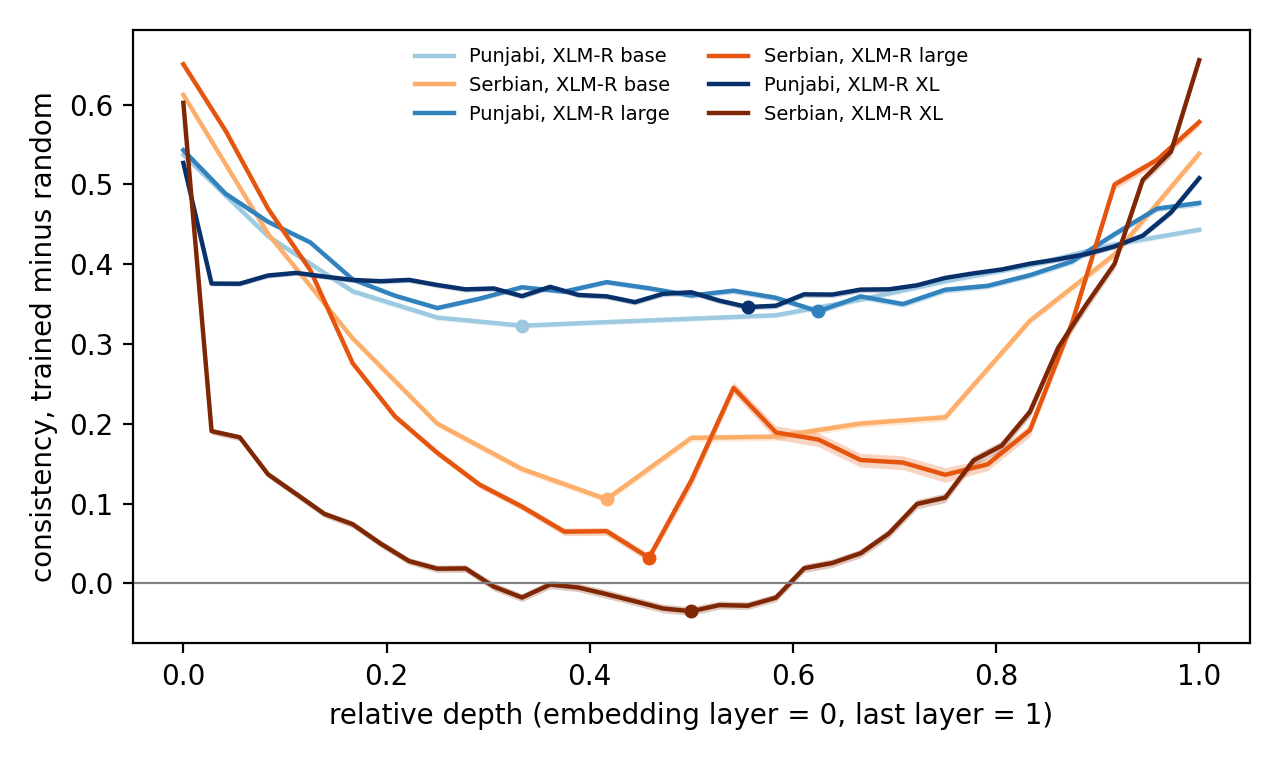
\includegraphics[width=0.9\textwidth,height=\textheight]{scale_depth.png}

\hypertarget{decoders}{%
\subsection{5.8 Decoders}\label{decoders}}

The three decoders of the main run (Qwen2.5-1.5B, Qwen2.5-3B and
Gemma-2-2B) were first pooled at the last token, and the result is
itself a finding. At the embedding layer the statistic then reduces to
the difference between two fixed punctuation embeddings: 1,941 of 2,009
FLORES sentences end in a full stop, and Gurmukhi and Shahmukhi use
different ones. A constant offset has consistency 1 by construction, and
trained and random-init models agree to two decimals (0.979 against
0.980 for Qwen2.5-1.5B) where the mean-pooled encoders differ sharply
(0.952 against 0.415 in XLM-R base). Serbian fails the other way, both
scripts ending in the same full stop, so the balanced pair is measured
on the zero vector. Finding 8 gives the full diagnosis.

We therefore reran all three with mean pooling and three random-init
seeds, on the same resample. None shows the encoder pattern. In both
Qwen2.5 models D for Punjabi rises with depth with no mid-stack trough
(from 0.040 at the embedding layer to 0.484 at the last in 1.5B), and
Serbian is separated more than Punjabi at every layer. At the middle
layer Serbian sits at 0.626 against Punjabi's 0.328 in 1.5B (difference
-0.299 {[}-0.315, -0.280{]}) and at 0.619 against 0.390 in 3B.
Gemma-2-2B is mixed. Serbian is separated more at the first ten and last
seven of its 27 depths, and Punjabi slightly more in between, by at most
0.05. In Qwen2.5-1.5B the script-form share is 0.966 {[}0.951, 0.979{]},
above every encoder.

One difference may matter. These vocabularies hold few Gurmukhi entries
(10 in Qwen2.5 and 144 in Gemma-2, against 1,675 in XLM-R, Section 3.6),
so Gurmukhi reaches them largely as bytes. We cannot separate that from
the other differences between the architectures. The decoders show that
the Punjabi-against-Serbian ordering holds in these encoders and fails
in these decoders.

\begin{center}\rule{0.5\linewidth}{0.5pt}\end{center}

\hypertarget{conclusion}{%
\section{6 Conclusion}\label{conclusion}}

Punjabi lets us hold language fixed and vary script. In four
multilingual encoders the two Punjabi scripts stay further apart than a
random network keeps them, through the lower and middle layers, on
generated and on human-written text. Graded controls leave 0.65 to 0.90
of that separation once information is matched, and the share falls at
every step as the bracket assumes. In a public recreation of XLM-R's
training data Shahmukhi Punjabi is about 1\% as frequent as Gurmukhi,
while Serbian's Latin orthography is abundant as Croatian and Bosnian.
Across three XLM-R sizes Serbian's two scripts move closer than a random
network keeps them and Punjabi's do not. That fits the idea that a
script with little closely related text resists abstraction. The two
pairs still differ in more than resource, and three decoders do not show
the ordering, so the claim is limited to these encoders. Transliteration
recovers 45\% of the accuracy lost in cross-script topic classification.
A design that varies script resource within one language would test the
explanation itself.

\hypertarget{limitations}{%
\section{7 Limitations}\label{limitations}}

\textbf{Data.} The FLORES Shahmukhi is machine-generated, and 7.4\% of
its sentences carry at least one error by human judgement (Section 3.5).
On human-written PuMVR text, generation inflates the Punjabi gap by
about a tenth (Section 5.6). The human set is smaller and
question-style. De-voweling matches information only approximately, and
the controls bracket an information-matched condition without
reproducing it. The Hindi-Urdu contrast carries a register confound.

\textbf{Resource.} The counts cover XLM-R only, since a recreation of
its training corpus is public. MuRIL's and the decoders' corpora are not
available in a form we can count. Both classifiers decide only lines
that contain marker words, and their error rates come from FLORES. Two
files were read in part and scaled up. The Serbian Latin estimate is a
lower bound, since Serbian written with ijekavian forms is counted as
Croatian. We measure resource and do not manipulate it.

\textbf{Scope.} The claims rest on four mean-pooled encoders. Three
mean-pooled decoders do not show the Punjabi-against-Serbian ordering
(Section 5.8). MuRIL's Serbian condition is not usable (13.4\% UNK).
Probes are at ceiling at every layer, so no depth claim rests on them.
The behavioural arm cannot compare scripts at the model sizes we tried.

\textbf{Statistics.} The bootstrap resamples sentences. Random-init seed
variation is checked separately, by repeating each ordering seed by seed
(Section 5.3). The intervals are tight enough that the no-script control
also excludes zero, with inconsistent signs across models, so effect
sizes carry more weight here than ``excludes zero'' does. Consistency is
stable under the additive nuisances of Section 4.2 and moves under some
content-script interactions. It reports the part of a script effect
shared across sentences. The script-form share is a ratio of nonlinear
statistics and no additive decomposition. The upper-layer recovery seen
on consistency does not survive a change of statistic, and we make no
claim from it.

\begin{center}\rule{0.5\linewidth}{0.5pt}\end{center}

\hypertarget{references}{%
\section{References}\label{references}}

Adelani, D. I., et al.~2024. SIB-200: A simple, inclusive, and big
evaluation dataset for topic classification in 200+ languages and
dialects. EACL.

Benjamini, Y., and Hochberg, Y. 1995. Controlling the false discovery
rate. Journal of the Royal Statistical Society B 57(1).

Conneau, A., et al.~2020. Unsupervised cross-lingual representation
learning at scale. ACL.

Gemma Team. 2024. Gemma 2: Improving open language models at a practical
size. arXiv:2408.00118.

Goyal, N., Du, J., Ott, M., Anantharaman, G., and Conneau, A. 2021.
Larger-scale transformers for multilingual masked language modeling.
RepL4NLP.

Hermjakob, U., May, J., and Knight, K. 2018. Out-of-the-box universal
romanization tool uroman. ACL System Demonstrations.

Hewitt, J., and Liang, P. 2019. Designing and interpreting probes with
control tasks. EMNLP-IJCNLP.

Jayakumar, T., Halder, D., and Dabre, R. 2026. Scripts through time: A
survey of the evolving role of transliteration in NLP. Findings of ACL.

Karne, S. 2026. One language, two scripts: Probing script-invariance in
LLM concept representations. arXiv:2603.08869.

Khanuja, S., et al.~2021. MuRIL: Multilingual representations for Indian
languages. arXiv:2103.10730.

Kornblith, S., Norouzi, M., Lee, H., and Hinton, G. 2019. Similarity of
neural network representations revisited. ICML.

Kudugunta, S., Bapna, A., Caswell, I., and Firat, O. 2019. Investigating
multilingual NMT representations at scale. EMNLP-IJCNLP.

Libovický, J., Rosa, R., and Fraser, A. 2020. On the language neutrality
of pre-trained multilingual representations. Findings of EMNLP.

Moosa, I. M., Akhter, M. E., and Habib, A. B. 2023. Does transliteration
help multilingual language modeling? Findings of EACL.

NLLB Team. 2022. No language left behind: Scaling human-centered machine
translation. arXiv:2207.04672. FLORES+ as maintained by the Open
Language Data Initiative.

Office of the Registrar General of India. 2011. Census of India 2011:
Language, Statement 1.

Pakistan Bureau of Statistics. 2023. Seventh Population and Housing
Census: Population by mother tongue.

Pires, T., Schlinger, E., and Garrette, D. 2019. How multilingual is
multilingual BERT? ACL.

Qwen Team. 2024. Qwen2.5 technical report. arXiv:2412.15115.

Rust, P., Pfeiffer, J., Vulić, I., Ruder, S., and Gurevych, I. 2021. How
good is your tokenizer? On the monolingual performance of multilingual
language models. ACL.

Shehzadi, A., Rauf, S. A., Malik, M. G. A., and Imran, M. 2024.
Unsupervised Punjabi corpus and neural machine transliteration system.
Manuscript cited by the SLPG model card as Heliyon, under review. We
were unable to locate a published version. The card reports 98.1 BLEU
and 99.5\% word accuracy for Gurmukhi to Shahmukhi. We could not
reproduce these figures because the preprocessing is undocumented
(Finding 6).

Singh, P., Pawar, B., Reddiboina, M., and Sheth, R. 2026. Not truly
multilingual: Script consistency as a missing dimension in VLM
evaluation. Findings of EMNLP. arXiv:2606.17188.

Song, L., Smola, A., Gretton, A., Bedo, J., and Borgwardt, K. 2012.
Feature selection via dependence maximization. JMLR 13.

Tang, T., et al.~2024. Language-specific neurons: The key to
multilingual capabilities in large language models. ACL.

Verma, A. A. K., Chatterjee, A., Gupta, M., and Chakraborty, T. 2026.
Multilingual language models encode script over linguistic structure.
ACL.

Wenzek, G., Lachaux, M.-A., Conneau, A., Chaudhary, V., Guzmán, F.,
Joulin, A., and Grave, E. 2020. CCNet: Extracting high quality
monolingual datasets from web crawl data. LREC.

Wu, S., and Dredze, M. 2019. Beto, bentz, becas: The surprising
cross-lingual effectiveness of BERT. EMNLP-IJCNLP.

\end{document}
